\section{Niveau 1}
\input{clerc/Anéantissement_de_la_peur_(Peur).tex}
\input{clerc/Détection_de_la_magie.tex}
\input{clerc/Détection_du_mal_(C).tex}
\vspace*{\fill}\columnbreak
\begin{spell}
\spellcarac{name}{Guérison des blessures légères}
\spellcarac{level}{1}
\spellcarac{duree}{Instantanée}
\spellcarac{portee}{Toucher}
\spellcarac{description}{

Ce sort a deux usages :
\begin{enumerate}
\item
  \textbf{Guérir une cible vivante :} Restaure 1d6+1 points de vie, sans dépasser le total maximum.
\item
  \textbf{Guérir la paralysie :} Annule les effets paralysants.
\end{enumerate}

\subsubsection{Inversé : Blessures légères}

Inflige 1d6+1 points de dégâts à une créature touchée. En combat, un jet
d'attaque de mêlée est nécessaire.
}
\end{spell}

\begin{spell}
\spellcarac{name}{Lumière}
\spellcarac{level}{1}
\spellcarac{duree}{12 tours}
\spellcarac{portee}{36 m}
\spellcarac{description}{Ce sort a trois usages :

\begin{enumerate}
\item
  \textbf{Invoquer une lumière magique :} Dans un rayon de 5 m. La lueur
  magique permet de lire, mais est moins vive que la lumière du jour. Le
  sort peut être lancé sur un objet, auquel cas la lumière se déplace
  avec lui.
\item
  \textbf{Aveugler une créature :} En lançant le sort directement sur
  ses yeux. Si la cible rate son jet de sauvegarde contre les sorts,
  elle perd l'usage de la vue pour la durée du sort. Une créature
  aveuglée est incapable d'attaquer.
\item
  \textbf{Annuler les ténèbres :} Lumière peut annuler le sort ténèbres
  (voir ci-dessous)
\end{enumerate}

\subsection{Inversé : Ténèbres}

Crée une zone d'obscurité magique dans un rayon de 5 m, privant toute
créature de sa vue normale (mais pas d'une éventuelle infravision). À la
manière de lumière, sa version réversible, ce sort peut servir à
aveugler une créature ou à annuler le sort lumière.
}
\end{spell}

\vspace*{\fill}\columnbreak
\begin{spell}
\spellcarac{name}{Protection contre le mal}
\spellcarac{level}{1}
\spellcarac{duree}{6 tours}
\spellcarac{portee}{Le lanceur}
\spellcarac{description}{Ce sort protège le lanceur des attaques de créatures d'un autre
alignement, comme suit :

\begin{itemize}
\item
  \textbf{Bonus :} Le lanceur reçoit un bonus de +1 à ses jets de
  sauvegarde contre les attaques et les capacités spéciales des
  créatures affectées.
\item
  \textbf{Attaques des créatures affectées :} Les attaques contre le
  lanceur se font avec un malus de --1 pour les créatures affectées.
\item
  \textbf{Créatures enchantées, artificielles ou convoquées :} En outre,
  le sort empêche les créatures enchantées, artificielles ou convoquées
  d'attaquer le lanceur en mêlée (mais pas à distance). Si le lanceur
  attaque une telle créature en mêlée, la protection est levée -- le
  lanceur conserve toutefois les bonus aux jets de sauvegarde et les
  malus à l'attaque indiqués ci-dessus.
\end{itemize}
}
\end{spell}

\input{clerc/Purification_de_l’eau_et_des_aliments.tex}
\vspace*{\fill}\columnbreak
\input{clerc/Résistance_au_froid.tex}

\vspace*{25pt}
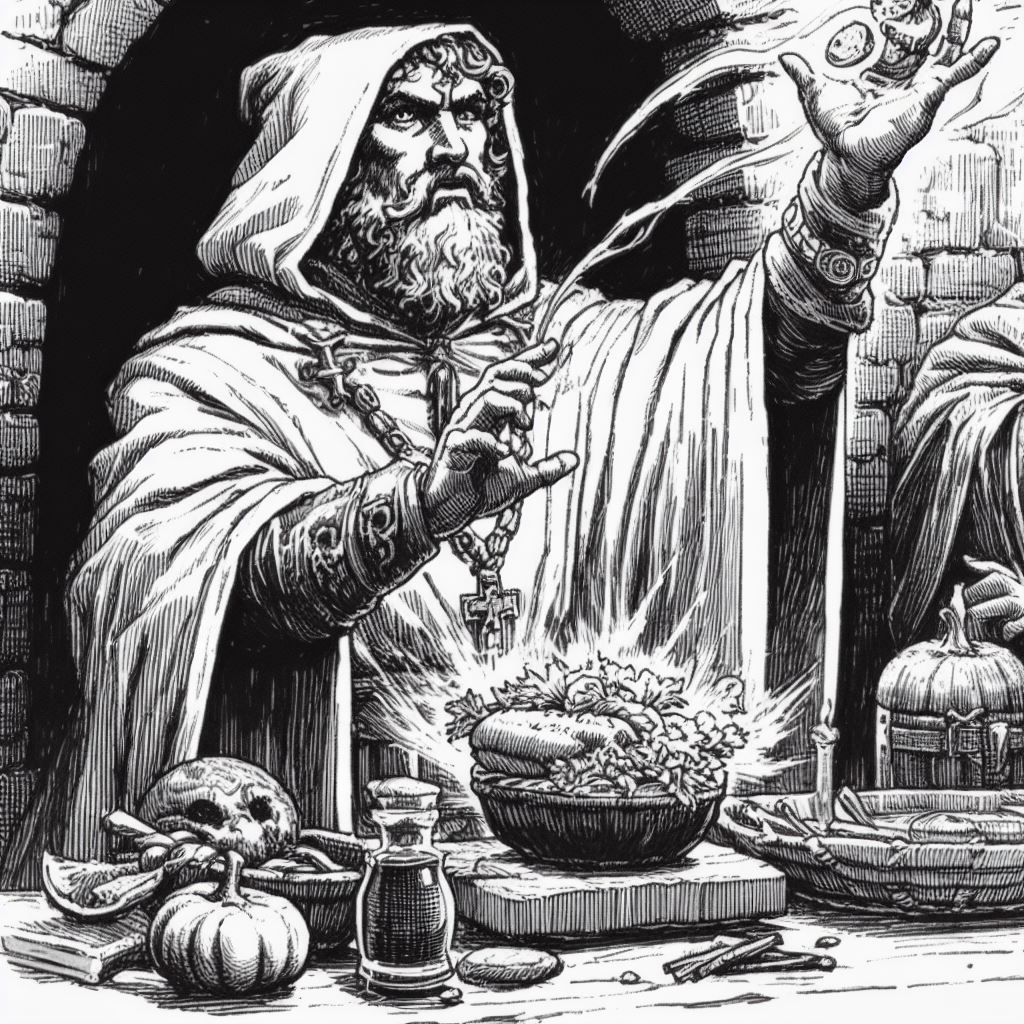
\includegraphics[width=\columnwidth]{img/purification.jpg}

\newpage
\section{Niveau 2}
\begin{spell}
\spellcarac{name}{Bénédiction}
\spellcarac{level}{2}
\spellcarac{duree}{6 tours}
\spellcarac{portee}{18 m}
\spellcarac{description}{Ce sort peut être utilisé dans l'une des deux situations suivantes :

\begin{enumerate}
\item
  \textbf{Combat :} Les alliés situés dans une zone de 6 m² et qui ne
  sont pas encore engagés en mêlée reçoivent un bonus à l'attaque et aux
  dégâts de +1, ainsi qu'un bonus de +1 à leur moral.
\item
  \textbf{Rituel :} À la discrétion de l'arbitre, le sort bénédiction
  peut faire partie de certains rituels de purification ou de
  consécration.
\end{enumerate}

\subsection{Inversé : Malédiction}

Ce sort entraîne un malus de --1 aux jets de moral, ainsi qu'aux jets
d'attaques et de dégâts dans une zone de 6m². Un jet de sauvegarde
contre les sorts est permis pour résister à malédiction.
}
\end{spell}

\begin{spell}
\spellcarac{name}{Charme-serpents}
\spellcarac{level}{2}
\spellcarac{duree}{1d4+1 rounds/tours}
\spellcarac{portee}{18 m}
\spellcarac{description}{Un ou plusieurs serpents cessent d'être hostiles. Ils se dressent et
ondulent, mais n'attaquent pas.

\begin{itemize}
\item
  \textbf{DV affectés :} Le sort charme un nombre de serpents dont le
  total de Dés de vie ne dépasse pas le niveau du lanceur. Par exemple,
  un lanceur de 7e niveau peut affecter 7 DV de serpents, ce qui
  équivaut à sept serpents de 1 DV chacun, ou un serpent de 3 DV et
  quatre serpents de 1 DV, ou toute autre combinaison.
\item
  \textbf{Durée :} Si le sort est lancé sur des serpents déjà en train
  d'attaquer, il dure 1d4+1 rounds. Autrement, le sort dure 1d4+1 tours.
\end{itemize}
}
\end{spell}

\begin{spell}
\spellcarac{name}{Détection des pièges}
\spellcarac{level}{2}
\spellcarac{duree}{2 tours}
\spellcarac{portee}{9 m}
\spellcarac{description}{Les objets et les zones piégés à portée émettent une lueur bleutée.

\begin{itemize}
\item
  \textbf{Pièges mécaniques et magiques :} Les deux types de pièges sont
  détectés.
\item
  \textbf{Aucune connaissance :} Le lanceur du sort n'apprend rien ni
  sur la nature de piège ni sur le moyen de le désamorcer.
\end{itemize}
}
\end{spell}

\vspace*{\fill}\columnbreak
\begin{spell}
\spellcarac{name}{Langage animal}
\spellcarac{level}{2}
\spellcarac{duree}{6 tours}
\spellcarac{portee}{9m}
\spellcarac{description}{Lorsque le sort est lancé, le lanceur peut communiquer avec un type
d'animal à portée.

\begin{itemize}
\item
  \textbf{Type d'animal :} Le sort fonctionne sur les animaux ordinaires
  tout comme leurs versions géantes.
\item
  \textbf{Questions :} Le lanceur peut poser des questions aux animaux
  du type choisi et recevoir d'eux des réponses. Mais le sort ne les
  rend pas plus amicaux ou coopératifs (un jet de réaction peut être
  nécessaire).
\item
  \textbf{Services :} Si l'animal est amical envers le lanceur, il peut
  lui accorder une faveur ou un service.
\end{itemize}
}
\end{spell}

\begin{spell}
\spellcarac{name}{Paralysie}
\spellcarac{level}{3}
\spellcarac{duree}{9 tours}
\spellcarac{portee}{36 m}
\spellcarac{description}{Ce sort paralyse un ou plusieurs humanoïdes qui ratent leur jet de sauvegarde contre les sorts.
Il peut être lancé de deux manières~:
\begin{enumerate}
\item \textbf{Contre un individu :} Le jet de sauvegarde de la cible se fait
  avec un malus de -2.
\item \textbf{Sur un groupe :} Le sort affecte 1d4 individus au sein du groupe.
\end{enumerate}

\textbf{Restrictions :} Les humanoïdes de plus de 4+1 DV et les
morts-vivants sont immunisés.
}
\end{spell}

\begin{spell}
\spellcarac{name}{Perception des alignements}
\spellcarac{level}{2}
\spellcarac{duree}{1 round}
\spellcarac{portee}{3 m}
\spellcarac{description}{Le lanceur connaît immédiatement l'alignement d'un personnage, d'un
monstre, d'un objet ou d'un lieu à portée. La plupart des objets et des
lieux sont dépourvus d'alignement, mais les objets magiques et les lieux
saints peuvent en avoir un.
}
\end{spell}

\vspace*{\fill}\columnbreak
\input{clerc/Résistance_au_feu.tex}
\vspace*{\fill}\columnbreak
\begin{spell}
\spellcarac{name}{Silence sur 5m}
\spellcarac{level}{2}
\spellcarac{duree}{12 tours}
\spellcarac{portee}{54 m}
\spellcarac{description}{Une zone dans un rayon de 5 m devient absolument silencieuse.

\begin{itemize}
\item
  \textbf{À l'intérieur de la zone :} Tous les sons sont stoppés. Il est
  impossible de se parler ou de lancer des sorts.
\item
  \textbf{Bruits extérieurs à la zone :} Les créatures à l'intérieur
  entendent les bruits provenant de l'extérieur de la zone.
\item
  \textbf{Lancé sur une créature :} Silence sur 5 m peut être lancé sur
  une créature, qui doit alors effectuer un jet de sauvegarde contre les
  sorts. Si elle rate, la zone de silence se déplace avec la cible. Si
  elle réussit, le sort reste fixe et la créature peut s'en extraire.
\end{itemize}
}
\end{spell}


%\newpage
\section{Niveau 3}
\begin{spell}
\spellcarac{name}{Contrecoup}
\spellcarac{level}{3}
\spellcarac{duree}{1 tour}
\spellcarac{portee}{9m}
\spellcarac{description}{
Enchante une arme :

\begin{itemize}
\item
  \textbf{Dégâts :} Elle inflige 1d6 points de dégâts supplémentaires.
\item
  \textbf{Considérée comme magique :} Elle est capable de blesser les
  monstres qui ne peuvent être blessés que par des armes magiques.
\end{itemize}
}
\end{spell}

\begin{spell}
\spellcarac{name}{Croissance animale}
\spellcarac{level}{3}
\spellcarac{duree}{12 tours}
\spellcarac{portee}{36m}
\spellcarac{description}{Un animal normal, non-magique, voit sa taille et sa force doublées après
que ce sort ait été lancé sur lui.

\begin{itemize}
\item
  \textbf{Dégâts :} Les dégâts infligés par l'animal sont doublés.
\item
  \textbf{Chargement :} Le poids que l'animal peut transporter sur lui
  est doublé.
\end{itemize}

\textbf{Restrictions :} Ce sort peut être utilisé sur les versions
géantes d'animaux normaux, mais les animaux intelligents et les monstres
fantastiques sont immunisés.
}
\end{spell}

\vspace*{\fill}\columnbreak
\begin{spell}
\spellcarac{name}{Désenvoûtement}
\spellcarac{level}{3}
\spellcarac{duree}{Instantané}
\spellcarac{portee}{Toucher}
\spellcarac{description}{Désenvoûtement ôte instantanément l'envoûtement d'une créature. Ce sort
peut permettre à un personnage de se débarrasser d'un objet magique
maudit.

\subsubsection{Inversé : Envoûtement}
Place un effet nocif sur une créature, si elle rate son jet de
sauvegarde contre les sorts.

\begin{itemize}
\item
  \textbf{Effets :} Forme et effets déterminés par le lanceur.
\item
  \textbf{Effets les plus graves possibles :} -2 aux jets
  de sauvegarde, -4 aux jets d'attaque, réduction d'une
  caractéristique de 50\%.
\item
  \textbf{Envoûtements multiples :} Peuvent affecter une créature tant
  que les effets de ces envoûtements sont différents.
\item
  \textbf{Décision de l'arbitre :} L'arbitre décide des effets de
  ce sort et peut retourner les envoûtements trop puissants sur le
  lanceur !
\item
  \textbf{Durée :} Permanent
\end{itemize}
}
\end{spell}

\vspace*{\fill}\columnbreak
\input{clerc/Guérison_des_maladies_(Contamination).tex}
\input{clerc/Localisation_d’objets_(C).tex}
\vspace*{\fill}\columnbreak
\begin{spell}
\spellcarac{name}{Lumière éternelle}
\spellcarac{level}{2}
\spellcarac{duree}{Permanente}
\spellcarac{portee}{36 m}
\spellcarac{description}{Ce sort a trois usages :

\begin{enumerate}
\item
  \textbf{Invoquer une lumière permanente :} Dans un rayon de 9 m. La
  lumière magique permet de lire, sans éclairer comme en plein jour pour
  autant. Le sort peut être lancé sur un objet, auquel cas la lumière se
  déplace avec ce dernier.
\item
  \textbf{Aveugler une créature :} En lançant ce sort sur ses yeux. Si
  la cible rate son jet de sauvegarde contre les sorts, elle est
  aveuglée. Une créature aveuglée est incapable d'attaquer.
\item
  \textbf{Annuler les ténèbres :} Lumière éternelle annule le sort
  ténèbres éternelles.
\end{enumerate}

\subsubsection{Inversé : Ténèbres éternelles}

Crée une zone de ténèbres magiques dans un rayon de 9 m, empêchant à la
fois la vision normale et l'infravision. Les sources de lumière à
l'intérieur de la zone de ténèbres ne l'éclairent pas. À la manière de
lumière éternelle, le sort peut aveugler une créature et annuler lumière
éternelle.
}
\end{spell}


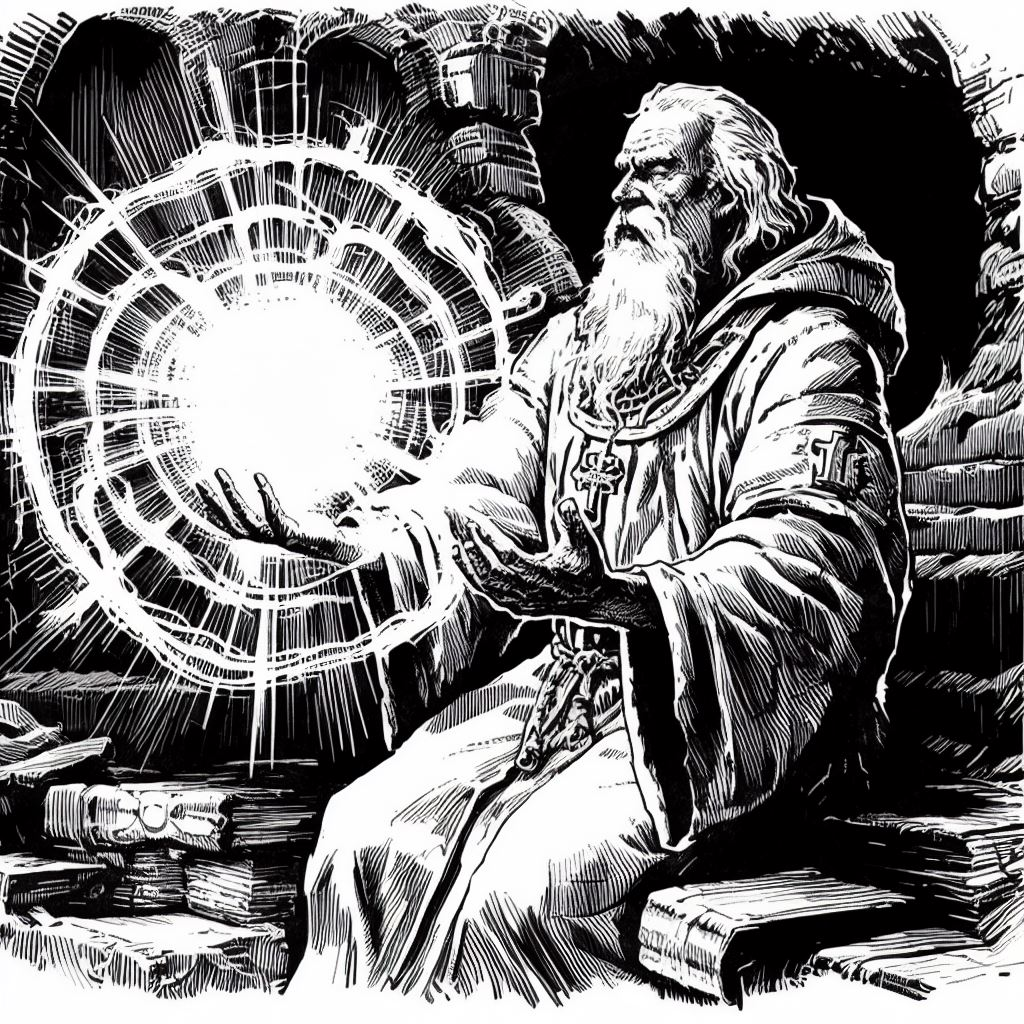
\includegraphics[width=\columnwidth]{img/lumiere.jpg}

\newpage
\section{Niveau 4}
\input{clerc/Aquagenèse.tex}
\begin{spell}
\spellcarac{name}{Bâtons à serpents}
\spellcarac{level}{4}
\spellcarac{duree}{6 tours}
\spellcarac{portee}{36m}
\spellcarac{description}{2d8 bouts de bois sont miraculeusement transformés en serpents qui
répondent aux ordres du lanceur.

\begin{itemize}
\item
  \textbf{Retour :} S'ils sont tués ou à la fin du sort, les serpents
  retournent à leur forme originelle de bouts de bois.
\end{itemize}
}
\end{spell}

\begin{spell}
\spellcarac{name}{Contre-poison}
\spellcarac{level}{4}
\spellcarac{duree}{Instantanée}
\spellcarac{portee}{Toucher}
\spellcarac{description}{Ce sort a deux usages :

\begin{enumerate}
\def\labelenumi{\arabic{enumi}.}
\item
  \textbf{Personnages :} Le sort neutralise les effets d'un poison sur
  un personnage. Le personnage décédé par empoisonnement peut être
  ramené à la vie si contre-poison est lancé dans les 10 rounds suivant
  sa mort.
\item
  \textbf{Objets :} Le sort retire le poison d'un objet.
\end{enumerate}
}
\end{spell}

\input{clerc/Guérison_des_blessures_graves_(Blessures_graves).tex}
\vspace*{\fill}\columnbreak
\begin{spell}
\spellcarac{name}{Langage des plantes}
\spellcarac{level}{4}
\spellcarac{duree}{3 tours}
\spellcarac{portee}{9 m}
\spellcarac{description}{Ce sort à deux usages :

\begin{enumerate}
\def\labelenumi{\arabic{enumi}.}
\item
  \textbf{Plantes normales :} La communication avec les plantes
  naturelles. Le lanceur peut poser des questions, recevoir des réponses
  et quémander de simples faveurs. Les plantes peuvent accepter si la
  requête est à leur portée. Par exemple, une large zone de plantes
  rampantes peut s'écarter pour créer un chemin libre permettant au
  lanceur et à ses alliés de traverser.
\item
  \textbf{Plantes monstrueuses :} La communication avec les monstres
  végétaux ou basés sur les plantes.
\end{enumerate}
}
\end{spell}

\begin{spell}
\spellcarac{name}{Protection vs mal (3m)}
\spellcarac{level}{3}
\spellcarac{duree}{12 tours}
\spellcarac{portee}{Lanceur}
\spellcarac{description}{Ce sort protège le lanceur et ses alliés sur 3 m des attaques de
créatures d'un autre alignement, comme suit :

\begin{itemize}
\item
  \textbf{Bonus :} Ceux qui sont protégés reçoivent un bonus de +1 à
  leurs jets de sauvegarde contre les attaques et les capacités
  spéciales des créatures affectées.
\item
  \textbf{Attaques des créatures affectées :} Les attaques contre ceux
  qui sont protégés se font avec un malus de --1 pour les créatures
  affectées.
\item
  \textbf{Créatures enchantées, artificielles ou convoquées :} En outre,
  le sort empêche de telles créatures d'attaquer en mêlée ceux qui sont
  protégés (mais pas à distance). Si une personne protégée attaque une
  telle créature en mêlée, la protection est levée -- ceux qui sont
  protégés conservent toutefois les bonus aux jets de sauvegarde et les
  malus à l'attaque indiqués ci-dessus.
\end{itemize}
}
\end{spell}

\begin{center}
  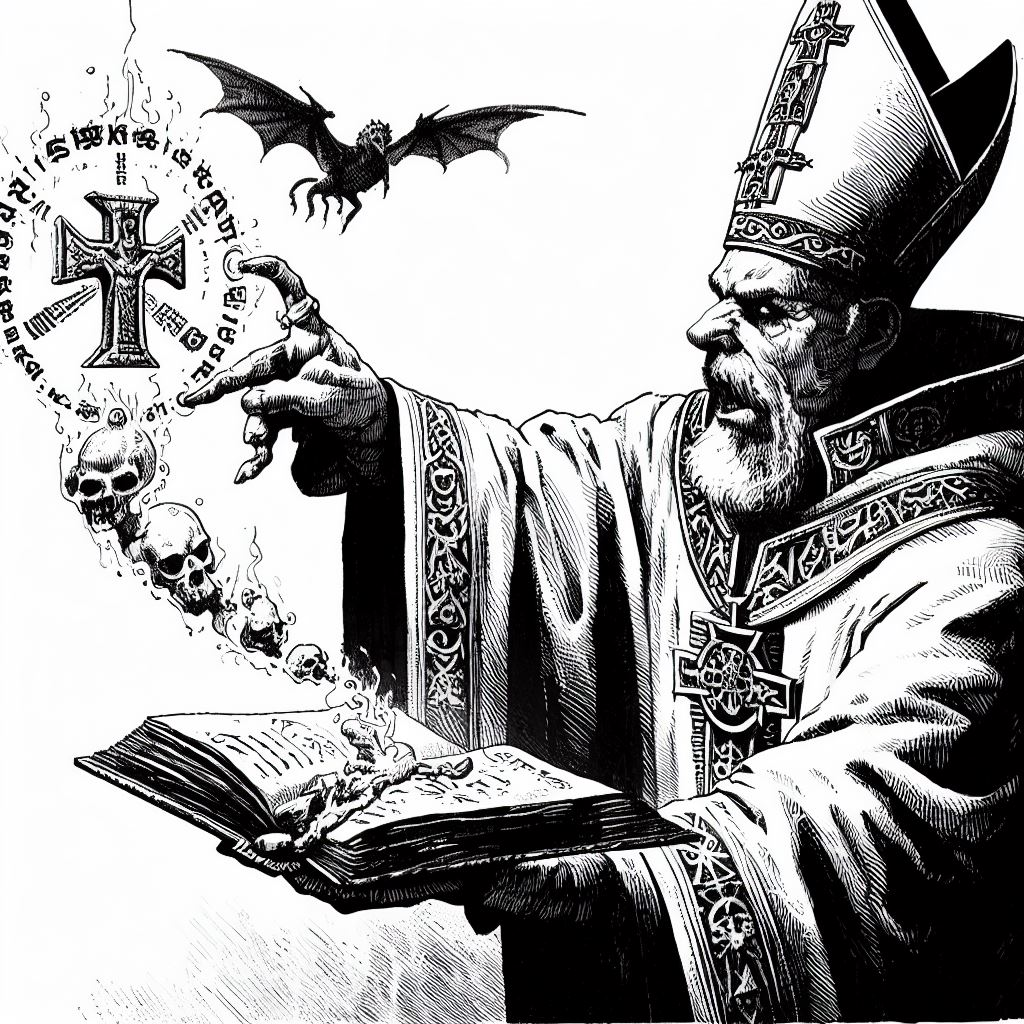
\includegraphics[width=0.8\columnwidth]{img/mal.jpg}
\end{center}

\newpage
\section{Niveau 5}
\begin{spell}
\spellcarac{name}{Communion}
\spellcarac{level}{5}
\spellcarac{duree}{3 tours}
\spellcarac{portee}{Le lanceur}
\spellcarac{description}{Le lanceur en appelle aux puissances divines pour acquérir des
connaissances.

\begin{itemize}
\item
  \textbf{Questions :} Le lanceur peut poser trois questions par sort
  lancé. Une fois par an, le lanceur peut à la place poser six
  questions.
\item
  \textbf{Réponses :} Chaque question reçoit comme réponse un simple «
  oui » ou « non ».
\item
  \textbf{Usage limité :} Communion ne peut être lancé qu'une fois par
  semaine. Si l'arbitre sent que ce sort est surutilisé, son usage peut
  être limité à une fois par mois.
\end{itemize}
}
\end{spell}

\input{clerc/Création_de_nourriture.tex}
\begin{spell}
\spellcarac{name}{Dissipation du mal}
\spellcarac{level}{5}
\spellcarac{duree}{1 tour}
\spellcarac{portee}{9 m}
\spellcarac{description}{description)

Ce sort a trois usages :

\begin{enumerate}
\item
  \textbf{Protection :} En restant concentré et immobile, les monstres
  enchantés et mort-vivants à portée peuvent être bannis ou détruits.
  Chaque monstre peut effectuer un jet de sauvegarde contre les sorts
  pour annuler le bannissement ou la destruction. Si le jet réussit, le
  monstre fuit la zone affectée.
\item
  \textbf{Cibler un seul monstre :} Bannit ou détruit instantanément un
  monstre enchanté ou mort-vivant à portée. Le monstre peut effectuer un
  jet de sauvegarde contre les sorts (avec un malus de --2) pour annuler
  le bannissement ou la destruction. Si le jet réussit, le monstre fuit
  la zone affectée.
\item
  \textbf{Désenvoûtement :} Dissipe instantanément l'empreinte qu'un
  objet maudit possède sur une cible vivante à portée.
\end{enumerate}
}
\end{spell}

\begin{spell}
\spellcarac{name}{Fléau d’insectes}
\spellcarac{level}{5}
\spellcarac{duree}{1 jour}
\spellcarac{portee}{144 m}
\spellcarac{description}{
Lancé au-dessus du sol, le sort invoque un essaim d'insectes volants de
18 m de diamètre, possédant les caractéristiques suivantes :

\begin{itemize}
\item
  \textbf{Déplacement :} 6 m par round. Tant que l'essaim est à portée,
  le lanceur peut diriger ses déplacements.
\item
  \textbf{Vision :} L'obscurité règne à l'intérieur de l'essaim.
\item
  \textbf{Créatures de 2 DV ou moins :} Si elles sont prises à
  l'intérieur de l'essaim, elles sont chassées.
\item
  \textbf{Concentration :} Si le lanceur se déplace ou perd sa
  concentration, l'essaim se dissipe, mettant fin au sort.
\end{itemize}

\textbf{Restrictions :} Le sort n'a aucun effet s'il est lancé sous
terre.
}
\end{spell}

\begin{spell}
\spellcarac{name}{Quête}
\spellcarac{level}{5}
\spellcarac{duree}{Permanent}
\spellcarac{portee}{9 m}
\spellcarac{description}{
Le lanceur impose à une cible unique d'effectuer une quête ou une tâche
spécifique.

\begin{itemize}
\item
  \textbf{Exemples :} Secourir un prisonnier, tuer un monstre
  spécifique, apporter un objet magique au lanceur ou effectuer un
  pèlerinage vers un lieu saint.
\item
  \textbf{Quête suicidaire :} La quête prescrite ne doit évidemment pas
  être manifestement suicidaire.
\item
  \textbf{Jet de sauvegarde :} La cible peut effectuer un jet de
  sauvegarde contre les sorts. Si elle réussit, quête n'a alors aucun
  effet.
\item
  \textbf{Refus :} La cible doit entreprendre la quête ou elle subit une
  malédiction (conformément au sort envoûtement, la nature exacte de la
  malédiction étant laissée à l'appréciation de l'arbitre).
\item
  \textbf{Accomplissement :} Une fois la tâche accomplie, le sort prend
  fin.
\end{itemize}

\subsection{Inversé : Annulation de quête}

Peut dissiper les effets d'un sort quête. Si la personne ayant lancé le
sort quête est d'un niveau supérieur à celle lançant le sort annulation
de quête, il est possible que ce dernier n'ait aucun effet. Les chances
d'échec sont de 5\% par niveau de différence entre les deux lanceurs.
}
\end{spell}

\vspace*{\fill}\columnbreak
\input{clerc/Rappel_à_la_vie_(Doigt_de_mort).tex}

\goOneColumns
\begin{figure}[hb]
  \centering
  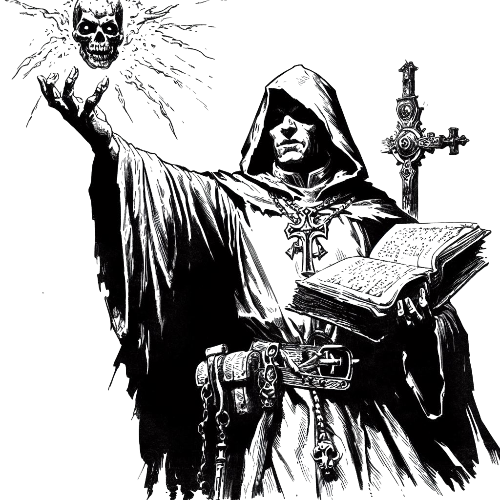
\includegraphics[width=0.8\columnwidth]{img/bad.png}
\end{figure}
\goTwoColumns

